\documentclass[size=a4, parskip=half, titlepage=false, toc=flat, toc=bib, 12pt]{scrartcl}

% ---------------------------------------------------------------------------
%  PAQUETES
% ---------------------------------------------------------------------------

% IDIOMA
\usepackage[utf8]{inputenc}

% MATEMÁTICAS
\usepackage{amsmath}    % Paquete básico de matemáticas
\usepackage{amssymb}	% Fuentes matemáticas
\usepackage{upgreek}
\usepackage{amsthm}     % Teoremas
\usepackage{mathrsfs}   % Fuente para ciertas letras utilizadas en matemáticas

% LISTAS
\usepackage{enumitem}       % Mejores listas
\setlist{leftmargin=.5in}   % Especifica la indentación para las listas.

% Dibujos Tikz
\usepackage{pgf,tikz}
\usepackage{tkz-euclide}
\usetkzobj{all}
\usepackage{mathrsfs}
\usetikzlibrary{arrows, calc,intersections,through,backgrounds}

% Títulos de figuras
\usepackage{capt-of}

% Posición de figuras
\usepackage{float}

% ---------------------------------------------------------------------------
%  RECURSOS
% ---------------------------------------------------------------------------

% Ruta donde buscar gráficos
\graphicspath{{../_assets/}, {_assets/}, {./img/}, {ALGI/img/}, {ALGI/}}

% ---------------------------------------------------------------------------
% ENTORNOS PERSONALIZADOS
% ---------------------------------------------------------------------------

%% DEFINICIONES DE LOS ESTILOS

% Nuevo estilo para definiciones
\newtheoremstyle{definition-style}  % Nombre del estilo
{}                                  % Espacio por encima
{}                                  % Espacio por debajo
{}                                  % Fuente del cuerpo
{}                                  % Identación
{\bfseries\sffamily}                      % Fuente para la cabecera
{.}                                 % Puntuación tras la cabecera
{.5em}                              % Espacio tras la cabecera
{\thmname{#1}\thmnumber{ #2}\thmnote{ (#3)}}  % Especificación de la cabecera

% Nuevo estilo para notas
\newtheoremstyle{remark-style}
{10pt}
{10pt}
{}
{}
{\itshape \sffamily}
{.}
{.5em}
{}

% Nuevo estilo para teoremas y proposiciones
\newtheoremstyle{theorem-style}
{}
{}
{}
{}
{\bfseries \sffamily}
{.}
{.5em}
{\thmname{#1}\thmnumber{ #2}\thmnote{ (#3)}}

% Nuevo estilo para ejemplos
\newtheoremstyle{example-style}
{10pt}
{10pt}
{}
{}
{\bfseries \sffamily}
{}
{.5em}
{\thmname{#1}\thmnumber{ #2.}\thmnote{ #3.}}

% Nuevo estilo para la demostración

\makeatletter
\renewenvironment{proof}[1][\proofname] {\par\pushQED{\qed}\normalfont\topsep6\p@\@plus6\p@\relax\trivlist\item[\hskip\labelsep\itshape\sffamily#1\@addpunct{.}]\ignorespaces}{\popQED\endtrivlist\@endpefalse}
\makeatother

%% ASIGNACIÓN DE LOS ESTILOS

% Teoremas, proposiciones y corolarios
\theoremstyle{theorem-style}
\newtheorem{nth}{Teorema}[section]
\newtheorem{nprop}{Proposición}[section]
\newtheorem{ncor}{Corolario}[section]
\newtheorem{lema}{Lema}[section]

% Definiciones
\theoremstyle{definition-style}
\newtheorem{ndef}{Definición}[section]

% Notas
\theoremstyle{remark-style}
\newtheorem*{nota}{Nota}

% Ejemplos
\theoremstyle{example-style}
\newtheorem{ejemplo}{Ejemplo}[section]

% Ejercicios y solución
\theoremstyle{definition-style}
\newtheorem{ejer}{Ejercicio}[section]

\theoremstyle{remark-style}
\newtheorem*{sol}{Solución}

% ---------------------------------------------------------------------------
% COMANDOS PERSONALIZADOS
% ---------------------------------------------------------------------------

% Números enteros: \ent
\providecommand{\ent}{\mathbb{Z}}

% Números racionales: \rac
\providecommand{\rac}{\mathbb{Q}}

% Números naturales: \nat
\providecommand{\nat}{\mathbb{N}}


% Valor absoluto: \abs{}
\providecommand{\abs}[1]{\lvert#1\rvert}

% Fracción grande: \ddfrac{}{}
\newcommand\ddfrac[2]{\frac{\displaystyle #1}{\displaystyle #2}}

% Texto en negrita en modo matemática: \bm{}
\newcommand{\bm}[1]{\boldsymbol{#1}}

% Línea horizontal.
\newcommand{\horrule}[1]{\rule{\linewidth}{#1}}

% Restricción de una aplicación.
\newcommand\restr[2]{{% we make the whole thing an ordinary symbol
  \left.\kern-\nulldelimiterspace % automatically resize the bar with \right
  #1 % the function
  \vphantom{\big|} % pretend it's a little taller at normal size
  \right|_{#2} % this is the delimiter
  }}

% Imagen de una aplicación.
\DeclareMathOperator*{\img}{img}

% Divisores de un elemento de un anillo
\DeclareMathOperator*{\rdiv}{div}

% Listas ordenadas con números romanos (i), (ii), etc.
\newenvironment{nlist}
{\begin{enumerate}
    \renewcommand\labelenumi{(\emph{\roman{enumi})}}}
  {\end{enumerate}}

% División por casos con llave a la derecha.
\newenvironment{rcases}
{\left.\begin{aligned}}
    {\end{aligned}\right\rbrace}


% ---------------------------------------------------------------------------
%  COLORES
% ---------------------------------------------------------------------------

\usepackage{xcolor}     % Permite definir y utilizar colores

\definecolor{50}{HTML}{FFEBEE}
\definecolor{300}{HTML}{E57373}
\definecolor{500}{HTML}{F44336}
\definecolor{700}{HTML}{D32F2F}
\definecolor{900}{HTML}{B71C1C}


\setuptoc{toc}{leveldown}

% Ajuste de las líneas y párrafos
\linespread{1.2}
\setlength{\parindent}{0pt}
\setlength{\parskip}{12pt}

% Español
\usepackage[spanish, es-tabla]{babel}

% Matemáticas
\usepackage{amsmath}
\usepackage{amsthm}

% Links
%\usepackage{hyperref}

% Fuentes
\usepackage{newpxtext,newpxmath}
\usepackage[scale=.9]{FiraMono}
\usepackage{FiraSans}
\usepackage[T1]{fontenc}

\defaultfontfeatures{Ligatures=TeX,Numbers=Lining}
\usepackage[activate={true,nocompatibility},final,tracking=true,factor=1100,stretch=10,shrink=10]{microtype}
\SetTracking{encoding={*}, shape=sc}{0}

\usepackage{graphicx}
\usepackage{float}

% Mejores tablas
\usepackage{booktabs}

\usepackage{adjustbox}

% COLORES

\usepackage{xcolor}

\definecolor{verde}{HTML}{007D51}
\definecolor{esmeralda}{HTML}{045D56}
\definecolor{salmon}{HTML}{FF6859}
\definecolor{amarillo}{HTML}{FFAC12}
\definecolor{morado}{HTML}{A932FF}
\definecolor{azul}{HTML}{0082FB}
\definecolor{error}{HTML}{b00020}

% ENTORNOS
\usepackage[skins, listings, theorems]{tcolorbox}

\newtcolorbox{recuerda}{
  enhanced,
%  sharp corners,
  frame hidden,
  colback=black!10,
	lefttitle=0pt,
  coltitle=black,
  fonttitle=\bfseries\sffamily\scshape,
  titlerule=0.8mm,
  titlerule style=black,
  title=\raisebox{-0.6ex}{\small RECUERDA}
}

\newtcolorbox{nota}{
  enhanced,
%  sharp corners,
  frame hidden,
  colback=black!10,
	lefttitle=0pt,
  coltitle=black,
  fonttitle=\bfseries\sffamily\scshape,
  titlerule=0.8mm,
  titlerule style=black,
  title=\raisebox{-0.6ex}{\small NOTA}
}

\newtcolorbox{error}{
  enhanced,
%  sharp corners,
  frame hidden,
  colback=error!10,
	lefttitle=0pt,
  coltitle=error,
  fonttitle=\bfseries\sffamily\scshape,
  titlerule=0.8mm,
  titlerule style=error,
  title=\raisebox{-0.6ex}{\small ERROR}
}

\newtcblisting{shell}{
  enhanced,
  colback=black!10,
  colupper=black,
  frame hidden,
  opacityback=0,
  coltitle=black,
  fonttitle=\bfseries\sffamily\scshape,
  %titlerule=0.8mm,
  %titlerule style=black,
  %title=Consola,
  listing only,
  listing options={
    style=tcblatex,
    language=sh,
    breaklines=true,
    postbreak=\mbox{\textcolor{black}{$\hookrightarrow$}\space},
    emph={jmml@UbuntuServer, jmml@CentOS},
    emphstyle={\bfseries},
  },
}

\newtcbtheorem[number within=section]{teor}{\small TEOREMA}{
  enhanced,
  sharp corners,
  frame hidden,
  colback=white,
  coltitle=black,
  fonttitle=\bfseries\sffamily,
  %separator sign=\raisebox{-0.65ex}{\Large\MI\symbol{58828}},
  description font=\itshape
}{teor}

\newtcbtheorem[number within=section]{prop}{\small PROPOSICIÓN}{
  enhanced,
  sharp corners,
  frame hidden,
  colback=white,
  coltitle=black,
  fonttitle=\bfseries\sffamily,
  %separator sign=\raisebox{-0.65ex}{\Large\MI\symbol{58828}},
  description font=\itshape
}{prop}

\newtcbtheorem[number within=section]{cor}{\small COROLARIO}{
  enhanced,
  sharp corners,
  frame hidden,
  colback=white,
  coltitle=black,
  fonttitle=\bfseries\sffamily,
  %separator sign=\raisebox{-0.65ex}{\Large\MI\symbol{58828}},
  description font=\itshape
}{cor}

\newtcbtheorem[number within=section]{defi}{\small DEFINICIÓN}{
  enhanced,
  sharp corners,
  frame hidden,
  colback=white,
  coltitle=black,
  fonttitle=\bfseries\sffamily,
  %separator sign=\raisebox{-0.65ex}{\Large\MI\symbol{58828}},
  description font=\itshape
}{defi}

\newtcbtheorem{ejer}{\small EJERCICIO}{
  enhanced,
  sharp corners,
  frame hidden,
  left=0mm,
  right=0mm,
  colback=white,
  coltitle=black,
  fonttitle=\bfseries\sffamily,
  %separator sign=\raisebox{-0.65ex}{\Large\MI\symbol{58828}},
  description font=\itshape,
  nameref/.style={},
}{ejer}

% CÓDIGO
\usepackage{listings}

% CABECERAS
\pagestyle{headings}
\setkomafont{pageheadfoot}{\normalfont\normalcolor\sffamily\small}
\setkomafont{pagenumber}{\normalfont\sffamily}

% ALGORITMOS
\usepackage[vlined,linesnumbered]{algorithm2e}

% Formato de los pies de figura
\setkomafont{captionlabel}{\scshape}
\SetAlCapFnt{\normalfont\scshape}
\SetAlgorithmName{Algoritmo}{Algoritmo}{Lista de algoritmos}

% BIBLIOGRAFÍA
%\usepackage[sorting=none]{biblatex}
%\addbibresource{bibliografia.bib}

\begin{document}

\renewcommand{\proofname}{\normalfont\sffamily\bfseries\small DEMOSTRACIÓN}

\title{Método de ranking para el diseño de un motor de búsqueda}
\subject{Trabajo fin de grado}
\author{Johanna Capote Robayna\\
    Doble Grado en Informática y Matemáticas}
\date{}
\publishers{\vspace{2cm}
\includegraphics[height=2.5cm]{UGR}\vspace{1cm}}
\maketitle

\newpage

\tableofcontents
\newpage

\section{Primera aproximación}

En primer lugar, para elegir que página web es la primera que mostramos en el buscador y establecer
un orden, nos basamos en la información que podemos extraer de la red (sitios, contenido, enlaces de una página web a otra).
Esta información la podemos reflejar en una matriz, por ejemplo si estamos estudiando la información de $n$ páginas llamadas $P1, \dots , Pn$,
podemos reflejar los enlaces entre una página $j$ a otra página $i$, escribiendo un $1$ en la entrada de la
matriz $m_{i,j}$ y en el caso de que no haya enlace escribir un $0$.

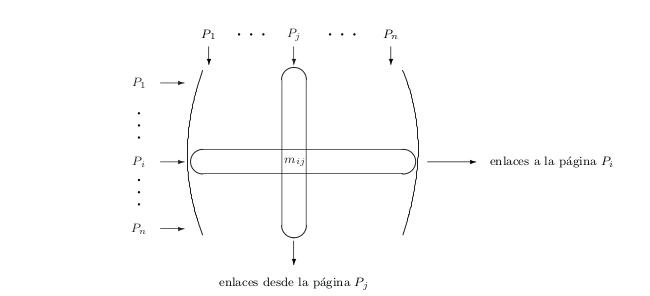
\includegraphics[width=1.0\textwidth]{./img/matriz}

Por lo tanto en la columna $j$ estarán los enlaces que salen de la página $P_j$ hacia otras páginas
mientras que en la fila $i$ estarán representados los enlaces a la página $P_i$. Por lo que esta matriz
no es simétrica ya que una página puede estar citada por otra y ella no citar a ninguna.

En una primera aproximación de querer ordenar las páginas web por ``importancia'' o ``relevancia'' podemos
pensar que la página a la que le lleguen más enlaces (fila con mayor número de $1$) es la que debería
mostrarse primero en el \textit{ranking}. Es decir si $x_j$ es la importancia de $P_j$, esta es proporcional
al número de páginas desde las que hay enlaces a $P_j$.

Sin embargo la realidad es que el número de enlaces a una cierta página no representa del todo su importancia,
ya que no es lo mismo que esta esté citada por una página cualquiera a que esté citada desde \verb|www.amazon.com| o
\verb|www.microsoft.com|. Estos dos últimos enlaces deberían ponderar más en importancia que otras citas de
otras páginas web menos relevantes. Por lo que para asignar importancia a una página web, deberemos tener
en cuenta tanto si es una página muy citada como si es una página poco citada, pero de sitio ``relevantes''.

Nos damos cuenta de la que importancia de la página citadora también es importante, por lo que pasamos a decir
que la importancia $x_j$ de una página $P_j$ es proporcional a la suma de las importancias de las páginas que enlazar
con $P_j$.

Supongamos, por ejemplo, que la página $P_1$ es citada desde las páginas $P_2$,$P_{25}$ y $P_{256}$,
 que $P_2$ sólo se cita desde $P_1$ y $P_{256}$, etc, mientas que en la última página $P_n$ hay enlaces
 desde $P_1$, $P_2$, $P_3$, $P_{25}$ y $P_{n-1}$. En nuestra asignación anterior, $x_1, \dots , x_n$ deberían
 cumplir entonces que:
 $$ x_1 = K (x_2 + x_{25} + x_{256}) $$
 $$ x_2 = K (x_1 + x_{256}) $$
 $$ \vdots $$
 $$x_n = K (x_1 + x_2 + x_3 + x_25 + x_{n-1}) $$

donde $K$ es una constante de proporcionalidad. Si nos fijamos, hemos construido un sistema de ecuaciones
donde las soluciones son los posibles valores de $x_1, \dots , x_n$. Este sistema de ecuaciones
lo podemos escribir en términos matriciales:

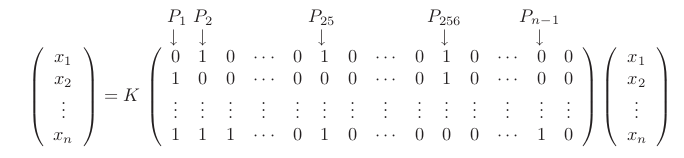
\includegraphics[width=1.0\textwidth]{./img/sde}

Si llamamos $X$ al vector de importacias $(x_1 \dots x_n)$, llamamos $\lambda = \frac{1}{K}$ y llamamos
$M$ a la matriz de dimensiones $n x n$ del sistema (matriz asociada al grafo). Nos encontramos
con un problema de autovaloes y autovectores:
$$Mx = \lambda x $$

A este vector $x$ le exigimos que sea no negativo, es decir $x \leq 0$ ya que representa la importancia
de una página web y también buscamos que sea único ya que como nuestro objetivo final es estrablecer un
\textit{ranking} de haber más de uno habría que diseñar otro proceso de selección.
El hecho de que el vector $x$ sea no negativo convierte a la matriz $M$ en no negativa ($M \leq 0$), ya que sus filas
están los valores $x_1, \dots , x_n$.

\begin{nth}[Perron, 1907]
Sea $A$ una matriz cuadrada ($A \in M_n(\mathbb{R})$) con estradas positivas, $A > 0$. Entonces:
\begin{enumerate}
\item Existe un autovalor (simple) \lamda > 0 tal que $Av = \lambda v$ donde el autovector es $v > 0$.
\item Este autovalor es mayor, en módulo, que todos los demás autovalores.
\item Cualquier otro autovector positivo de $A$ es un múltiplo de $v$.
\end{enumerate}
\end{nth}

Este teorema demostrado por Perron demostraría la existencia y unicidad de nuestro vector solución $x$,
sin embargo nuestra matriz $M$ puede tener entradas nulas por lo que no nos serviría el resultado.

\begin{ndef}[Matriz irreducible]
Se dice que una matriz $A \in M_n(\mathbb{R})$ es irreducible, cuando cumple alguna de las siguientes:
\begin{enumerate}
\item No existe ninguna permutación (de filas y columnas) que transforma $A$ en una matriz del tipo:
\begin{center}
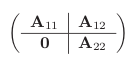
\includegraphics[width=0.2\textwidth]{./img/mcuadrada}
\end{center}
donde $A_{11}$ y $A_{22}$ son matrices cuadradas.
\item La matriz $(I + A)^{n - 1}$, donde $I$ es la identidad $n x n$, tiene todas sus entradas positivas.
\item Si $A$ es la matriz de adyacencia de un grafo, entonces el grafo está fuertemente conectado.
\end{enumerate}
\end{ndef}

\begin{nth}[Frobenius, 1908-1912]
Sea $A $ una matriz cuadrada con entradas no negativas ($A \leq 0$). Si $A$ es irreducible, entonces:
\begin{enumerate}
\item Existe un autorvalor (simple) $\lambda > 0$ tal que $A v = \lambda v$, donde el autovector es
$v > 0$. Además, $\lambda \leq |\mu|$, para cualquier otro autorvalor $\mu$ de $A$.
\item Cualquier autovector $\leq 0$ es múltiplo de $v$.
\item Si hay $k$ autovalores de módulo máximo, entonces son las soluciones de $x^k - \lambda^k = 0$.
\end{enumerate}
\end{nth}

¿¿FALTARÍA DEMOSTRAR QUE LA MATRIZ M ES UNA MATRIZ DE ADYACENCIA DE UN GRAFO FUERTEMENTE CONECTADO??
%printbibliography

\end{document}
